\usetikzlibrary{patterns}
\usetikzlibrary{fadings}
\usetikzlibrary{external}
\usetikzlibrary{calc}
\usetikzlibrary{positioning}
\usepgfplotslibrary{colormaps}
\usetikzlibrary{arrows}
\usetikzlibrary{matrix}

\usetikzlibrary{trees}


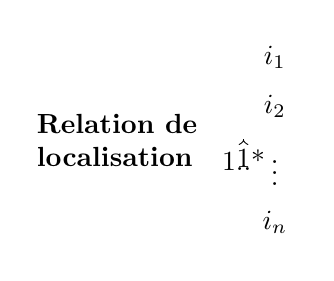
\begin{tikzpicture}
  \tikzset{
    acc/.style={decorate,decoration={brace,raise=0cm,amplitude=.1cm}},
    accm/.style={acc,decoration={mirror}},
    acc3/.style={acc,decoration={amplitude=.2cm}},
    acc3m/.style={acc3,decoration={mirror}}
  }
  
%% Matrices
\node[font=\bfseries, baseline, text width=2.5cm] (I) at (0,0) {Relation de localisation};

\matrix [matrix of math nodes,row sep=0.1cm,column sep=0.1cm,
anchor=west, nodes={anchor=base, baseline}] (is) at (I.east)
{i_1\\i_2\\\vdots{}\\i_n\\};

\draw[->, black] (I.east) -- (is.west) node[pos=0,below] {1} node[pos=1,below]{1..*};

\end{tikzpicture}